\chapter{Пути и графы}
% Читает КК.

\setlength{\epigraphwidth}{.53\textwidth}
\epigraph{Человеку приятен небольшой беспорядок в собственной геометрии.}{--- Луи де Берньер (1954---)}

%Человеку нравится неаккуратность в его геометрии

%Louis de Bernieres (2012). “Corelli's Mandolin: A Novel”, p.256, Vintage:

%The captain clicked his tongue disapprovingly, `Symmetry is only a property of dead things.
%Did you ever see a tree or a mountain that was symmetrical?
%It's fine for buildings, but if you ever see a symmetrical human face, you will have the impression that you ought to think it beautiful, but that in fact you find it cold.
%The human heart likes a little disorder in its geometry, Kyria Pelagia.
%Look at your face in a mirror, Signorina, and you will see that one eyebrow is a little higher than the other, that the set of the lid of your left eye is such that the eye is a fraction more open than the other.
%It is these things that make you both attractive and beautiful, whereas . . . otherwise you would be a statue. Symmetry is for God, not for us.'

%– Симметрия свойственна только мертвому. Вы когда-нибудь видели симметричные дерево или гору? Это хорошо для строений, а вот если бы вы увидели симметричноечеловеческое лицо, у вас бы сложилось впечатление, что его только полагается считать красивым, а на самом деле оно холодное. Человеческой душе нравится, чтобы в ее геометрии был небольшой беспорядок, кирья Пелагия. Посмотрите на себя в зеркало, синьорина, и вы увидите, что одна бровь у вас немного выше другой, что левое веко делает этот глаз чуточку шире. Но вы привлекательны и красивы, несмотря на... а иначе вы были бы статуей. Симметрия – для Господа, не для нас.

Спустимся в одномерный мир --- к кривым, которые вам должны быть известны, и графам, о которых вы, возможно, не слышали.
Граф --- это набор точек, называемых вершинами, некоторые пары из которых образуют \emph{рёбра}.
Часто вершины графа изображаются точками на плоскости, а его рёбра --- отрезками или кривыми, соединяющими одну свою вершину с другой.
Если при этом можно обойтись без пересечений рёбер друг с другом, то граф называется \emph{планарным}.

\subsection*{Укрепление сетки}\rindex{Укрепление сетки}

Дана сетка размера $n \times n$ из стержней единичной длины, шарнирно соединённых в концах.
Разрешается укрепить некоторые $S$ клеток диагональными скобами (длиной $\sqrt{2}$).

Какое количество $S$ достаточно для того, чтобы сделать сетку жёсткой на плоскости?

\begin{figure}[ht!]
\centering
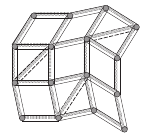
\includegraphics[scale=1]{pics/lattice1}
\caption{Недоукреплённая сетка.}
\label{pic:lattice1}
\end{figure}

На рис. \ref{pic:lattice1} показана недоукреплённая сетка $3 \times 3$.

\begin{addedbytheeditors}
Разумеется, речь идёт о минимально возможном значении $S$. Как всегда в подобных случаях, полное решение задачи включает не только пример с найденным $S$, но и оценку, показывающую, что меньшим $S$ достичь жёсткости сетки не удастся.  
\end{addedbytheeditors}

\subsection*{Путешествие по острову}\rindex{Путешествие по острову}

Алоизий катается по острову на своём прекрасном автомобиле.
Известно, что на каждом перекрёстке острова сходится ровно три (двусторонних) улицы.
Алоизий придерживается следующего правила:
начав с какого-то перекрёстка, он едет в произвольном направлении, на следующем перекрёстке он поворачивает направо, затем налево,
снова направо, налево, и так далее.

Докажите, что рано или поздно Алоизий вернётся на перекрёсток, с которого начал.

\parit{Примечания.}
Граф, в котором к каждой вершине подходят ровно три ребра, называется \emph{кубическим}.
В нашем графе есть понятия \emph{право} и \emph{лево},
для этого достаточно изобразить граф на плоскости, с рёбрами (улицами), образованными кривыми.
При этом не требуется \emph{планарность} графа;
в нём могут быть мосты и туннели, то есть места, где рёбра проходят друг над другом.

\subsection*{Провода под Гудзоном}\rindex{Провода под Гудзоном}

Пятьдесят одинаковых проводов проведены под рекой Гудзон.
Нужно определить все пары концов на обоих берегах.
Для этого разрешается замыкать любые пары проводов на западном берегу, а на восточном проверять концы;
другими словами, вы можете выяснить, какие пары проводов на восточном берегу соединены на западном.

Сколько потребуется поездок через Гудзон, чтобы справиться с этим заданием?

\subsection*{Жуки на четырёх прямых}\rindex{Жуки на четырёх прямых}

Даны четыре прямые общего положения на плоскости (никакие две не параллельны и никакие три не пересекаются в одной точке).
Вдоль каждой прямой ползёт жук-призрак с постоянной скоростью (скорости разных жуков могут быть разными).
Будучи призраками, при встрече жуки продолжают ползти сквозь друг друга.

Докажите, что если произошли пять из всех шести возможных встреч,
то была и шестая.

\medskip

Ну раз уж мы начали про жуков...

\subsection*{Пауки на кубе}\rindex{Пауки на кубе}

Три паука и муравей бегают по рёбрам куба.
Каждый паук бегает втрое медленней муравья.
Докажите, что пауки смогут поймать муравья.

\medskip

Следующая головоломка знакомит нас с прекрасной теоремой теории графов.

\subsection*{Вменяемые мыслители}\rindex{Вменяемые мыслители}\label{Вменяемые мыслители}

Жители Перевёртовска каждую неделю встречаются и обсуждают городские дела, в частности, поддерживать ли им строительство нового торгового центра.
Во время встреч каждый перевёртовец обсуждает этот вопрос со всеми своими друзьями (у каждого их нечётное число), а на следующий день (если требуется) он меняет своё мнение о торговом центре так, чтоб оно совпадало со мнением большинства его друзей.

Докажите, что начиная с какого-то момента, каждую \emph{вторую} неделю у каждого перевёртовца будет то же самое мнение.

\parit{Примечания.}
Очевидно, что рано или поздно произойдёт зацикливание, ведь существует только конечное число наборов мнений (их $2^n$, если в городе $n$ жителей). 
В данном случае утверждается, что период цикла должен быть $2$ (или $1$).
С чего бы это?

\medskip

И под конец задача о ком-то, кто хотел бы остаться на своём графе.

\subsection*{Лемминг на шахматной доске}\rindex{Лемминг на шахматной доске}\label{Лемминг на шахматной доске}

На каждой клетке шахматной доски $n\times n$ поставлена стрелка к одной из  восьми соседних клеток (или за пределы доски, если это клетка на краю),
причём направления стрелок в соседних клетках (включая диагональные) могут различаться не более чем на $45^\circ$.

Лемминг стартует с центральной клетки и идёт по стрелкам.
Придётся ли ему упасть с доски?

\begin{addedbytheeditors}
Здесь спрашивается, существует ли такая расстановка стрелок, при которой лемминг упадёт с доски? 
\end{addedbytheeditors}